\documentclass[12pt,a4paper]{article}
\usepackage[utf8]{inputenc}
\usepackage{amsmath}
\usepackage{amsfonts}
\usepackage{amssymb}
\usepackage{graphicx}
\usepackage{subcaption}
\usepackage{float}
\usepackage{multirow}
\usepackage{rotating}

\author{Team Gamma \\ {\small Ajda Frankovič, Martin Preradović, Niki Bizjak}}
\title{Face recognition}
\date{}
\begin{document}
    \maketitle

    For our third task we were training a classifier to recognize twenty-one different faces, one face of Gargamel and twenty faces of women. We divided this task into three parts.

    \begin{enumerate}
      \item Obtaining training data
      \item Training different classifiers
      \item Evaluating the performance of the trained classifiers
    \end{enumerate}

    \section{Preparing training data}

    This was the most time consuming part in this task. We had to capture images of faces, crop them and then convert them into embeddings for training our classifiers.

    \subsection{Capturing images of faces}

    For training the classifiers we decided to capture two sets of photos, to best replicate the conditions in the real world and in the gazebo simulation:

    \begin{enumerate}
      \item The first set of images was obtained with a physical camera. We printed the faces on A4 sheets of paper and captured photos of them under different lighting conditions and viewing angles. We obtained around 650 images of this kind.
      \item The second set of face images was obtained in the gazebo simulation. We drove the robot around the map, detected faces on the walls and saved them as images. We obtained around 950 images of this kind.
    \end{enumerate}    

    Here are the examples of our captured images.

    % add 4 photos of Gargamel from gazebo here and to the folder "images"
    \begin{figure}[H]
        \centering
        \includegraphics[width=.20\linewidth]{images/gargamel_outside_30_2m.jpg}
        \includegraphics[width=.20\linewidth]{images/gargamel_outside_0_15m.jpg}
        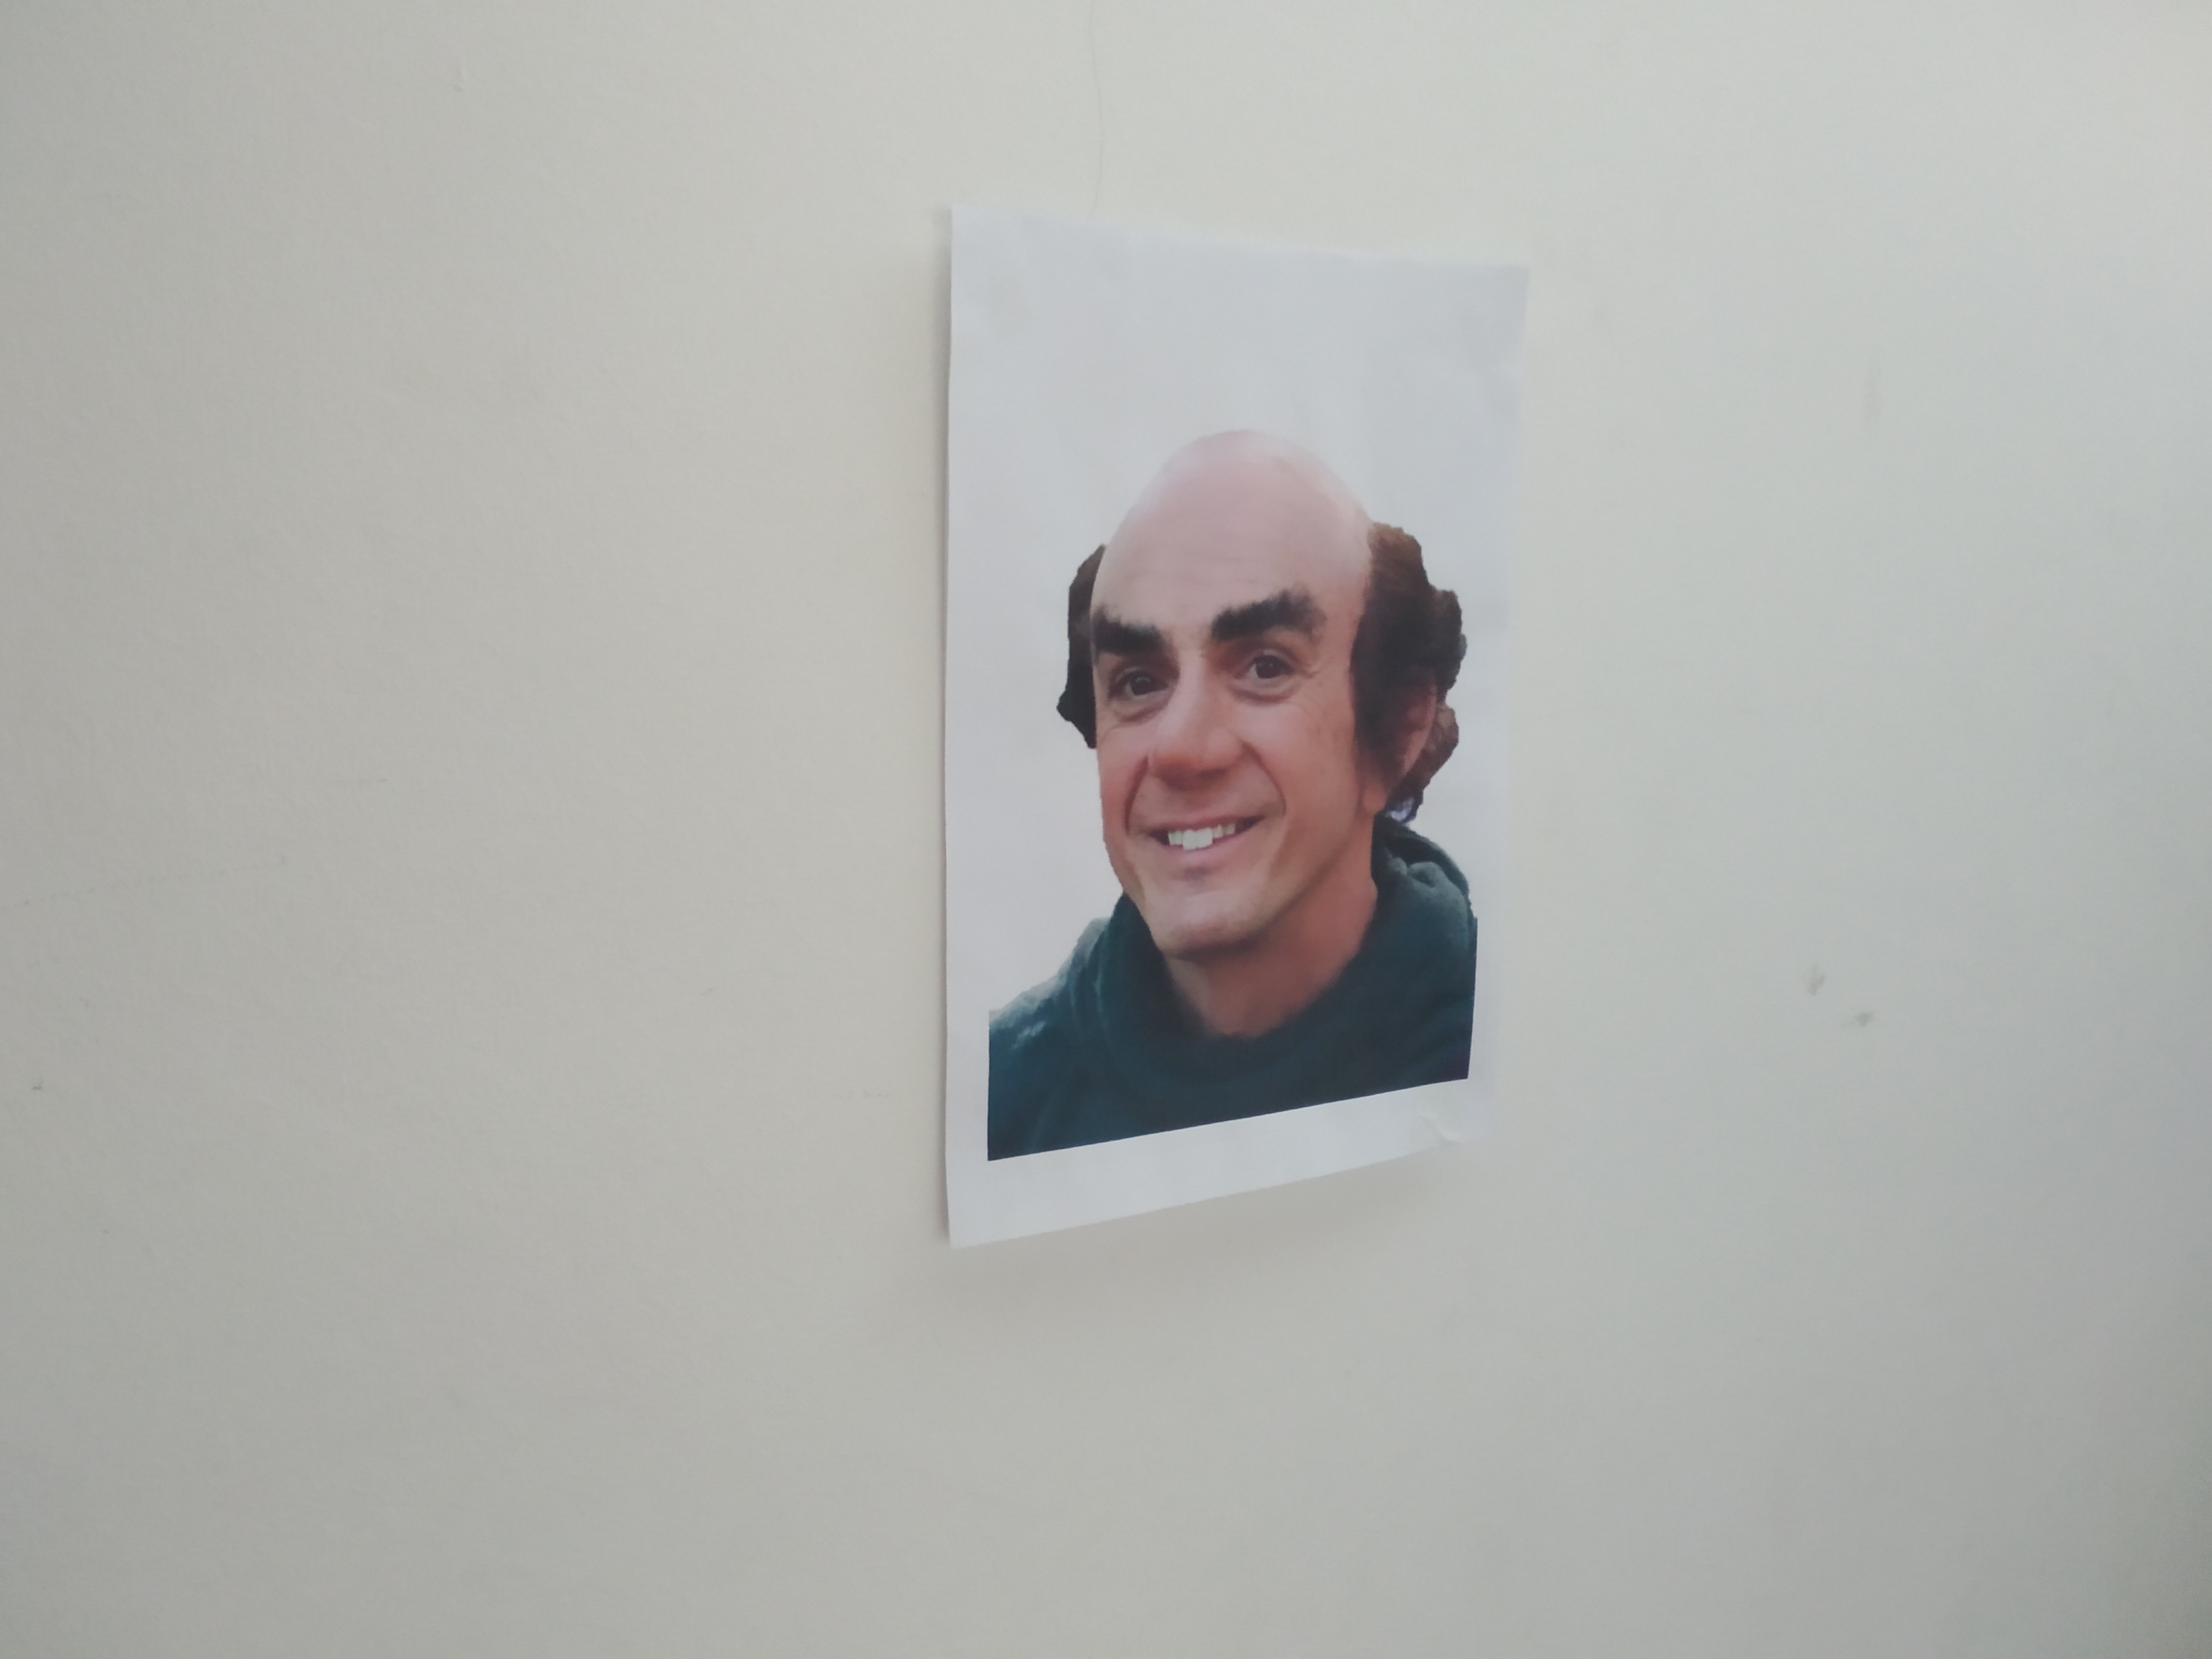
\includegraphics[width=.20\linewidth]{images/gargamel_inside_30_light.jpg}
        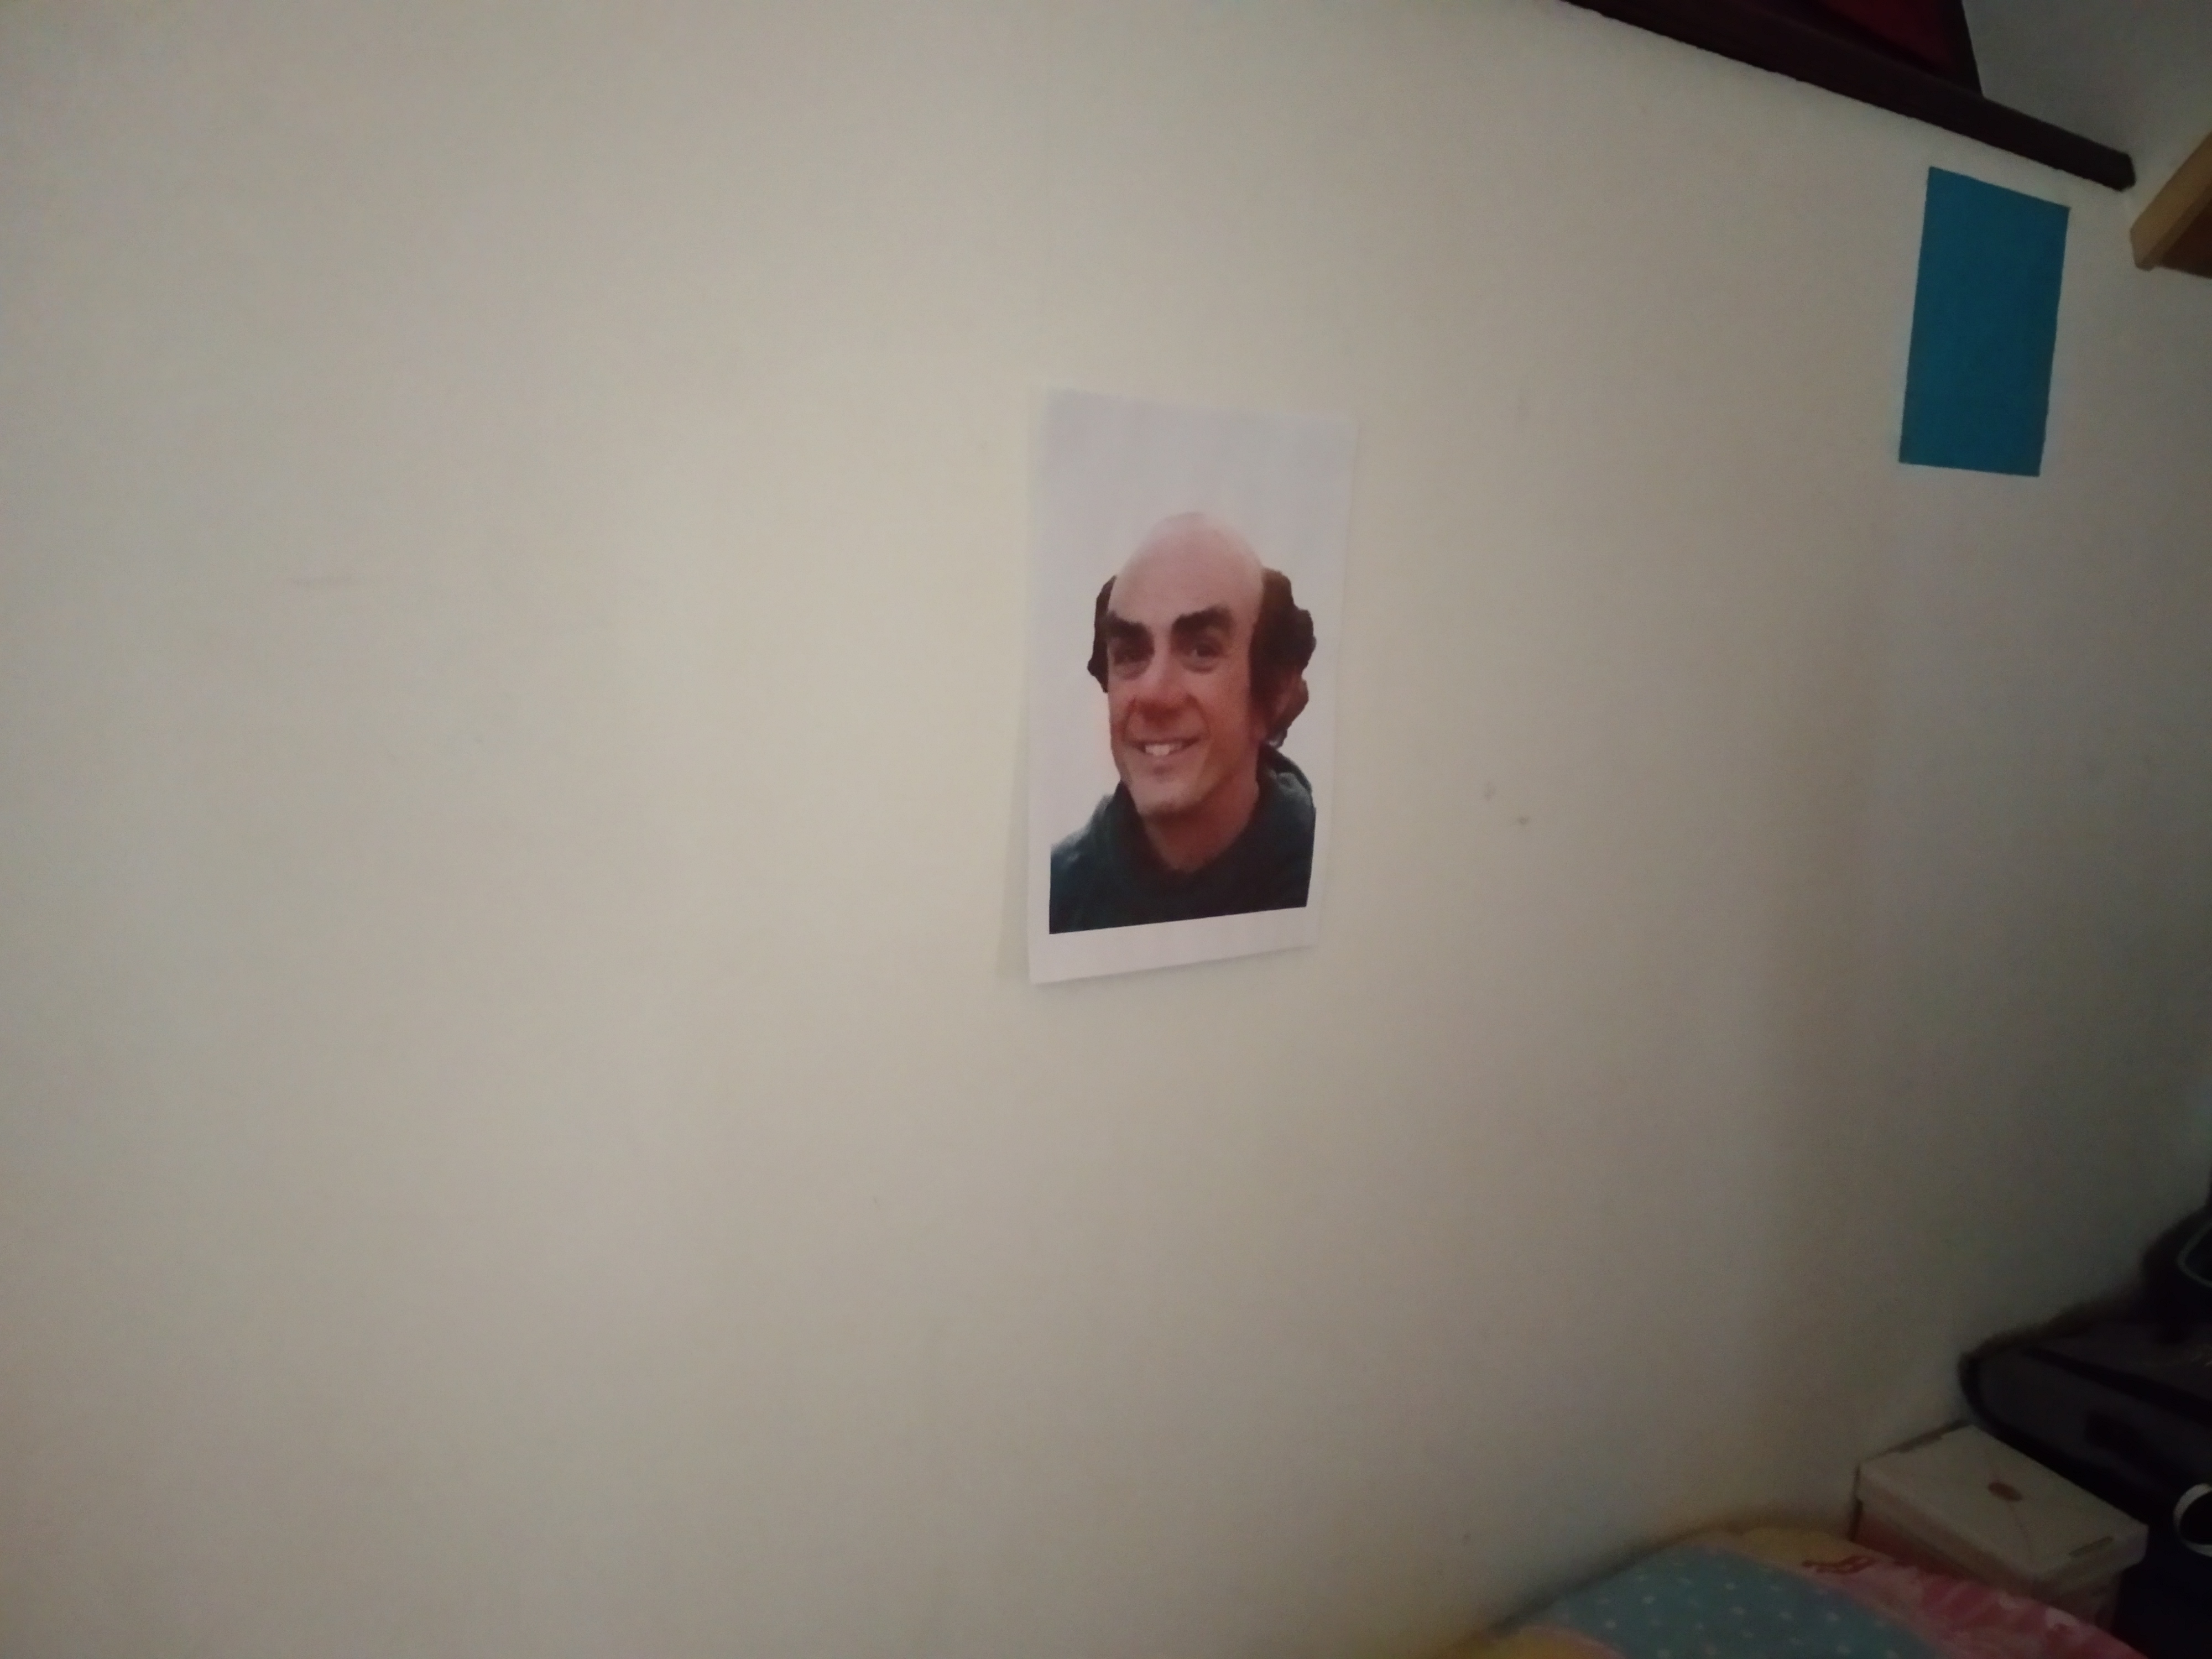
\includegraphics[width=.20\linewidth]{images/gargamel_inside_30_dark.jpg} \\
        \vspace{3pt}
        
\includegraphics[width=.20\linewidth]{images/gargamel_simulation_01.jpg}
        
\includegraphics[width=.20\linewidth]{images/gargamel_simulation_02.jpg}
        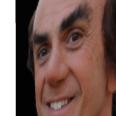
\includegraphics[width=.20\linewidth]{images/gargamel_simulation_03.jpg}
        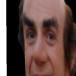
\includegraphics[width=.20\linewidth]{images/gargamel_simulation_04.jpg}
        \caption{Images of faces}
    \end{figure}

    \subsection{Preprocessing images}

    This step was relatively easy. We first detected the faces with our face detector, that we created for homework 1. Then we cropped the images to obtain faces. \\

    Note: This first step of detecting and cropping the faces was not necessary for the second set of our images, i.e. the ones taken in the gazebo simulator. That is because our pipeline for detecting faces in ros already includes cropping the faces out of the image. All we had to do in this case was to just save the photos and label them. \\

    We then fed the images to a python module named \texttt{face\_recognition} to obtain encodings, these are actually 128 dimensional vectors, that represent our faces. We saved these encodings into csv files along with labels of the faces for each encoding. \\

    The main reason for using this model over others is, that it is very straightforward and easy to use. It enables us to load the images and create encodings in just a few lines. The second reason being, that the model is very powerful and accurate, since in the background it actually uses \texttt{dlib}s state-of-the-art face recognition built with deep learning. \\

    Before using the encodings for training, we normalized them to increase classification accuracy mainly on knn and svm classifiers. Normalization of features had the biggest impact on svm models. \\

    \section{Face recognition}

    With our datasets ready, we then trained different classifiers to recognize faces and computed their accuracy. We envisioned three different approaches. \\

    First, we trained and tested our models only on encodings of faces that were captured in the simulation. This way we can best adjust the models to the conditions in the simulation and achieve the best classification accuracy for our task of recognizing faces. \\

    Second, we trained and tested our models only on encodings of faces that were captured with the camera in a physical world. This approach ensured that our models could also be trained to work in rougher conditions, for example under more complex lighting setting and blur that is usually present in photographs, that is not simulated in the gazebo simulator. \\

    Third, we wanted to see how the models will behave if we trained them with both datasets at once. This approach ensured, that our models could accurately classify faces in the simulation, but could also perform well in more diverse conditions. \\

    \subsection{Model selection}

    We are mainly interested in these three classifiers: knn, naive bayes and linear svm. \\

    We chose knn because it is a standard and very simple model, that is easy to understand. We don't, however, expect it to perform particularly well on this task because of high dimensionality of our data. \\

    The second model, naive bayes is also a standard model. It is very fast and easy to predict new the class of new data and it performs well in multi-class prediction. That is why we expect it to perform well. \\

    The third model that we are interested in is support vector machine. This is a standard and very accurate and robust classifier that is often used in smaller datasets where deep learning approaches aren't feasible. It also performs very well on large feature spaces, that is why we expect this classifier to be very effective for our task. \\

    We have also included some other classifiers such as decision tree and random forest to see how well they perform, out of curiosity. 

    \section{Evaluating performance}

    We then tested the classifiers using the datasets. All of our approaches were successful and we achieved more than 98\% accuracy on most of the classifiers. 

    Below is a table containing average classification accuracies of models for the three different approaches, that is three different train and test sets.

    \begin{center}
        \begin{tabular}{|c|c|c|c|}
            \hline
			 & \multicolumn{3}{c|}{\textbf{Partition into training and testing set}} \\
			\hline 
			\textbf{Classifier} & \texttt{Approach 1} & \texttt{Approach 2} & \texttt{Approach 3} \\
            \hline \hline
            
			\textbf{knn}, \small k = 1 & 0.995 & 1.000 & 0.987 \\
			\textbf{knn}, \small k = 3 & 0.995 & 0.978 & 0.979 \\
			\textbf{knn}, \small k = 5 & 0.995 & 0.956 & 0.962 \\
			\hline \hline
			\textbf{decision tree}, \small gini & 0.853 & 0.626 & 0.824 \\
			\textbf{decision tree}, \small entropy & 0.884 & 0.700 & 0.812 \\
			\hline \hline
			\textbf{random forest}, \small gini & 0.997 & 0.960 & 0.958 \\
			\textbf{random forest}, \small entropy & 0.996 & 0.981 & 0.965 \\
			\hline \hline
			\textbf{naive bayes} & 0.995 & 0.933 & 0.873 \\
			\hline \hline
			\textbf{svm}, \small kernel=linear, c=0.05 & 1.000 & 1.000 & 0.987 \\
			\textbf{svm}, \small kernel=linear, c=0.1 & 1.000 & 1.000 & 0.983 \\
			\textbf{svm}, \small kernel=linear, c=0.2 & 1.000 & 1.000 & 0.983 \\
			\hline
		\end{tabular} \\
    \end{center}

    We can see that all models perform extremely well on all three datasets, the only exception being decision tree, but it still works fairly well. \\

    There are a few reasons why the classifiers are so accurate.

    \begin{enumerate}
      \item The \texttt{face\_recognition} library does a very good job at encoding the faces. Seemingly it divides the images in the embedding space very well, as even the knn classifier performs good on this high dimensional data.
      \item Classification task requires us to recognize only twenty-one faces.
      \item The conditions in the simulation that we previously noted, i.e. lighting and absence of blur, make this task easier.
    \end{enumerate}

    Contrary to our prediction, the knn models perform incredibly well. We speculate that one reason for this is good separation of face encodings in the embedding. And the other reason might be, that even though encodings have 128 features, that is still a relatively small feature space, as for some machine learning tasks we can have datasets with 10.000 features or more. \\

    We also tried all knn versions with added weights (distance) but there was no noticeable difference in results, hence we omitted them. \\

    As we expected the support vector machine models work very well except for the one that uses a radial basis function (rbf) kernel. We can see that linear svm models perform similarly for all three values of c. \\

    We can observe that the naive bayes classifier performs worse than knn, which is surprising, but it is still more accurate than decision tree. \\

    Here we see a confusion matrix for the naive bayes classifier on the first dataset. We can observe that there are very few mistakes. Confusion matrix for the svm classifiers on the first dataset will not be shown, because it predicted every case correctly. Gargamel is represented as \texttt{face01}.
    
    \begin{figure}[H]
		\centering
		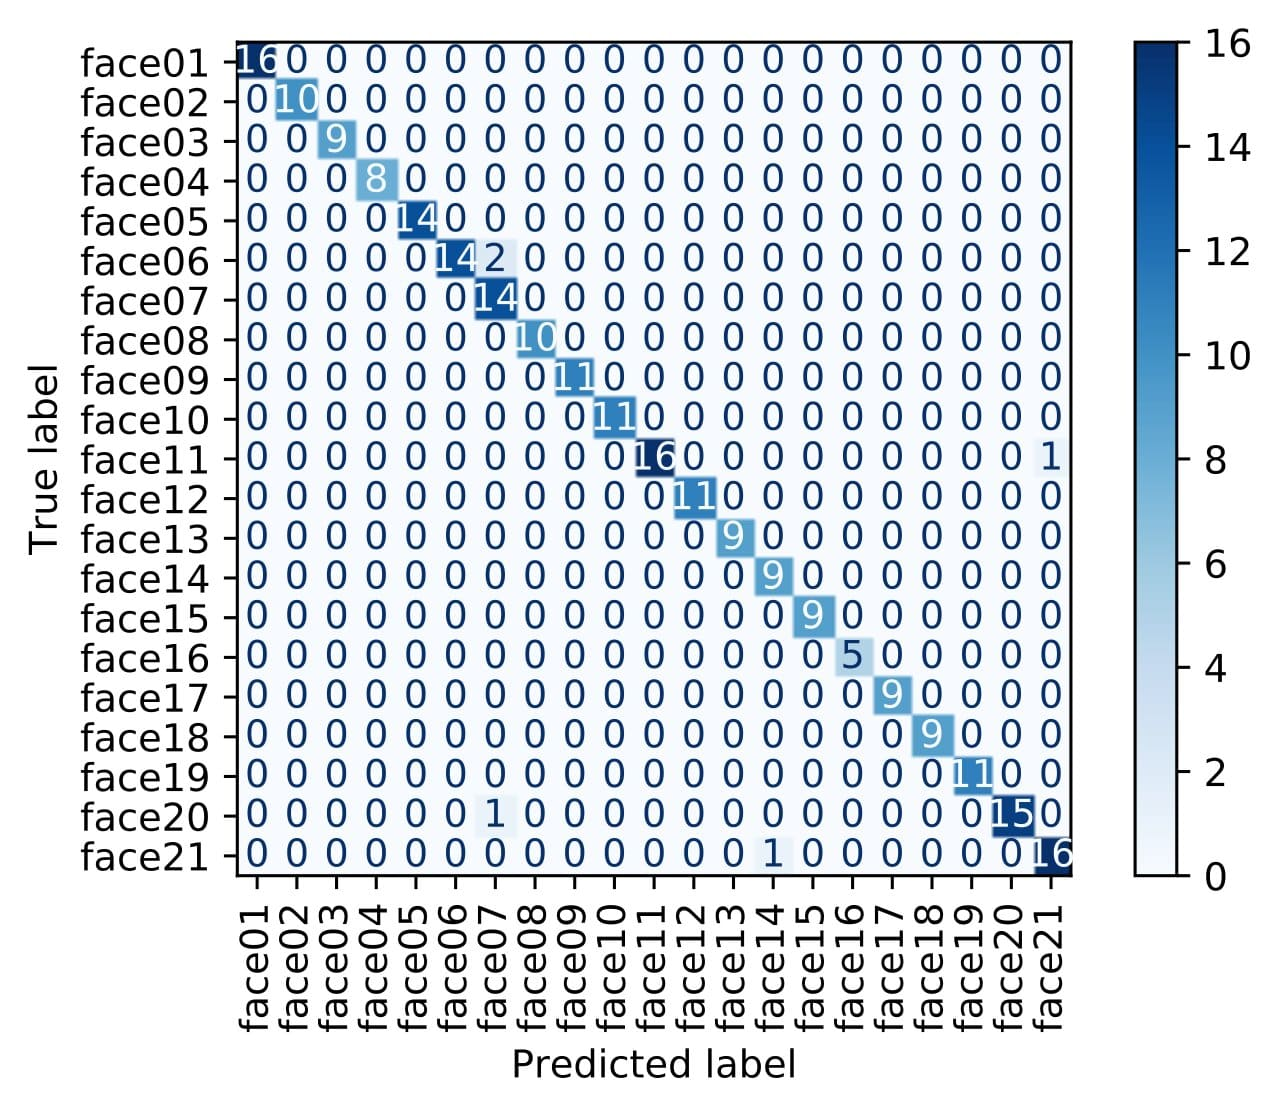
\includegraphics[width=1\linewidth]{images/naive_bayes_confusion_matrix.jpg}
		\caption{Confuson matrix for naive bayes classifier used on the first dataset partition}
    \end{figure}

    Since this is a multiclass confusion matrix, we read it a bit differently than the binary ones. This is explained in a picture below.

    \begin{figure}[H]
      \centering
      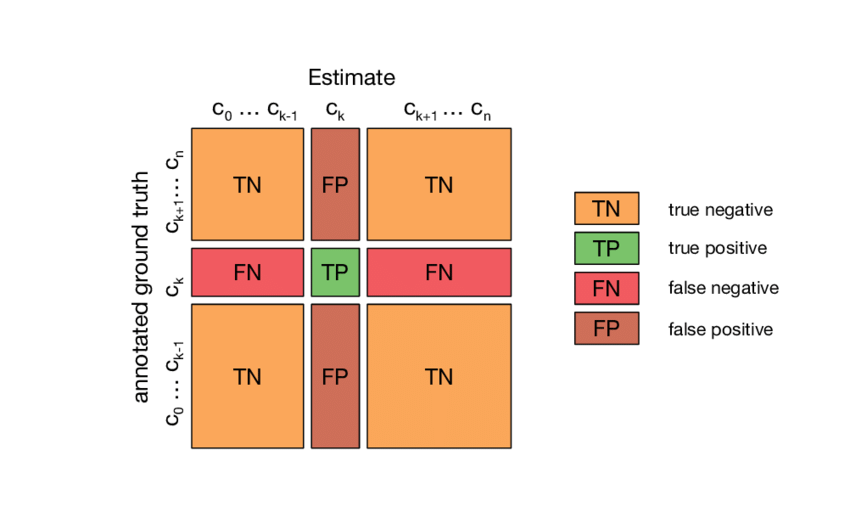
\includegraphics[width=1\linewidth]{images/Confusion_matrix_explanation.png}
      \caption{Multiclass confusion matrix, source: \small \textit{Activity, Context, and Plan Recognition with Computational Causal Behaviour Models - Scientific Figure on ResearchGate}}
    \end{figure}

    \section{Conclusion}

    Based on our results we have a few candidates to use for face recognition. Knn, svm, naive bayes and random forest. \\

    We choose the support vector machine model with a linear kernel and $C=0.05$, because it overall performed best in all three approaches. \\

    For the training dataset in task 3 we choose only the images taken in the simulation, because in this way we best adapt the classifier to the conditions in the gazebo simulator.
    
\end{document}